\documentclass[10pt]{article}
\usepackage{amsmath}
\usepackage{amsfonts}
\usepackage{amssymb}
\usepackage{graphicx}
\usepackage[margin=1in]{geometry}
\usepackage[labelfont=bf,labelsep=period]{caption}
\usepackage{booktabs}
\usepackage{multirow}
\usepackage{subcaption}

\title{Monte Carlo as Approximate Polynomial Preconditioning within MCSA}
\author{Steven Hamilton and Tom Evans and Stuart Slattery}

\newcommand{\bx}{\ensuremath{\mathbf{x}}}
\newcommand{\by}{\ensuremath{\mathbf{y}}}
\newcommand{\bb}{\ensuremath{\mathbf{b}}}
\newcommand{\bc}{\ensuremath{\mathbf{c}}}
\newcommand{\br}{\ensuremath{\mathbf{r}}}
\newcommand{\bp}{\ensuremath{\mathbf{p}}}
\newcommand{\bw}{\ensuremath{\mathbf{w}}}
\newcommand{\bA}{\ensuremath{\mathbf{A}}}
\newcommand{\bH}{\ensuremath{\mathbf{H}}}
\newcommand{\bM}{\ensuremath{\mathbf{M}}}
\newcommand{\bP}{\ensuremath{\mathbf{P}}}
\newcommand{\bW}{\ensuremath{\mathbf{W}}}
\newcommand{\bI}{\ensuremath{\mathbf{I}}}
\newcommand{\bK}{\ensuremath{\mathbf{K}}}
\newcommand{\calK}{\ensuremath{\mathcal{K}}}

\DeclareMathOperator*{\argmin}{arg\,min}

\begin{document}
\maketitle

\section{Background}
\label{sec:background}

Monte Carlo Synthetic Acceleration (MCSA), as described in Ref.~\cite{evans_13},
is an approach for solving the linear system
\begin{equation}
\bA \bx = \bb \label{eq:lin_problem}
\end{equation}
using a Monte Carlo (stochastic) process.
The original MCSA algorithm can be written as
\begin{equation}
\begin{aligned}
\bx^{k+1/2} &= \bx^{k} + \br^{k} \\
\bx^{k+1} &= \bx^{k+1/2} + \bM^{-1}\br^{k+1/2} \:,
\end{aligned}
\end{equation}
where $\bM^{-1}$ denotes performing an approximate linear solve using the
adjoint Monte Carlo process and $k$ is the iteration index.
Thus, MCSA consists of a single unpreconditioned
Richardson iteration followed by a single preconditioned Richardson iteration.
This iteration scheme has been observed to exhibit far better convergence
behavior than the original sequential Monte Carlo scheme proposed by Halton \cite{halton_94}.

The adjoint Monte Carlo process works by approximating the Neumann
series of the inverse of \bA:
\begin{equation}
\bA^{-1} = \sum_{n=0}^{\infty} ( \bI - \bA )^n
\equiv \sum_{n=0}^{\infty} \bH^n \:, \label{eq:neumann_inv}
\end{equation}
where \bH\ is the Richardson iteration matrix.
Correspondingly, the solution to a linear system of equations can
be written as
\begin{equation}
\bx = \sum_{n=0}^{\infty} \bH^n \bb \:. \label{eq:neumann_soln}
\end{equation}
Clearly
Eqs.~\eqref{eq:neumann_inv} and \eqref{eq:neumann_soln} are only
valid if the spectral radius of
the iteration matrix, $\rho(\bH)$, is less than unity.
The Monte Carlo process is conducted by decomposing the transpose of
\bH\ into an element-wise
(Hadamard) product of a probability matrix and a weight matrix, i.e.
\begin{equation}
\bH^T = \bP \circ \bW \:. \label{eq:mc_decomp}
\end{equation}
The usual approach is to define rows of \bP\ as normalized rows of $\bH^T$
(normalized columns of \bH), i.e.
\begin{equation}
\bP_{ij} =
\frac{\vert \bH_{ji} \vert}{\displaystyle \sum_{i=1}^{N} \vert \bH_{ij} \vert} \:.
\end{equation}
With this definition for \bP, the weight matrix is given by
\begin{equation}
\bW_{ij} = \frac{\bH_{ji}}{\bP_{ij}}. \label{eq:wgt_mat}
\end{equation}
Note that both \bP\ and \bW\ should have the same sparsity pattern
as $\bH^T$ and so Eq.~\eqref{eq:wgt_mat} is only taken over the indices corresponding
to nonzero entries in $\bH^T$.
The solution to a system of equations is approximated by following
a number of particle histories (although we are considering arbitrary
linear systems here, the nomenclature of tracking ``particles'' is
carried over from the particle transport community)
and averaging the contributions
to the solution over all conducted histories.  Each history is started
in a state determined by normalizing \bb to produce a probability
distribution:
\begin{equation}
\bp_i^\text{start} =
\frac{\vert \bb_i \vert}{\displaystyle \sum_{i=1}^{N} \vert \bb_i \vert} \:.
\end{equation}
The initial weight of a history is therefore given by
\begin{equation}
\bw_i^\text{start} = \frac{\bb_i}{\bp_i^\text{start}} \:.
\end{equation}
The history proceeds by allowing the particle to transition
to a new state by sampling from the discrete probability distribution
defined by the row of \bP\ corresponding to the current state.
The weight of the particle is updated by multiplying by the
entry in \bW\ corresponding to the given transition.
Each history provides a contribution to the solution vector proportional
to the current weight of the particle.  Either collision or
expected value tallies are possible, see [cite Slattery] for details
about these tally methods.
A given history can either be terminated via a weight cutoff (i.e.
when the weight of a particle drops below a prescribed fraction
of its initial weight) or by a history length cutoff (i.e. after
a certain number of transitions have taken place).

\section{Monte Carlo as Approximate Polynomial Preconditioning}
\label{sec:polynomial_prec}

As described in the previous section, the original idea behind
the adjoint Monte Carlo approach is to approximate the
Neumann series applied to the vector \bb.
However, by applying a history length cutoff it is possible to
view the Monte Carlo random walk as an approximation of a
fixed degree polynomial in $\bH$:
\begin{equation}
p(\bH) = \sum_{n=0}^{N} c_n \bH^n \:, \label{eq:neumann_poly}
\end{equation}
where in the standard algorithm, $c_n=1$.
The Neumann series is not the only polynomial that can approximate
$\bA^{-1}$, however.  By varying the selection of $c_n$, it is
possible to use other polynomials.  Commonly, polynomials used
for preconditioning are defined in terms of powers of \bA\ rather
than powers of \bH, giving the expansion
\begin{equation}
p(\bA) = \sum_{n=0}^{N} \hat{c}_n \bA^n \:. \label{eq:power_poly}
\end{equation}
Converting between coefficients defined by Eq.~\eqref{eq:power_poly}
and those defined by Eq.~\eqref{eq:neumann_poly} can be
accomplished by means of a change of basis.  The impact of the
choice of the basis will be evaluated in Section~\ref{sec:results}.
We now consider several candidates for the matrix polynomial.

\subsection{Chebyshev Polynomials}
\label{subsec:chebyshev}

One approach to defining a preconditioner, $\bM$, is to
attempt to minimize the eigenvalues of $\bI - p(\bA) \bA$.
The Chebyshev polynomials, denoted $T_m(x)$ have the property
that out of all monic polynomials of degree $m$,
$\frac{1}{2^{m-1}} T_m(x)$ is the polynomial whose maximum
absolute value is minimized over the interval $[-1,1]$.
Thus, if the spectrum of \bA is real, then an optimal polynomial
preconditioner can be achieved by mapping the eigenvalues of
\bA\ into the interval $[-1,1]$ using the transformation
\begin{equation}
\ell (\bA) = \alpha \bI + \beta \bA \:,
\end{equation}
where $\alpha  \equiv -\dfrac{\lambda_\text{max} + \lambda_\text{min}}
{\lambda_\text{max} -  \lambda_\text{min}}$,
$\beta \equiv \dfrac{2}{\lambda_\text{max} -  \lambda_\text{min}}$,
and $\lambda_\text{min}$ and $\lambda_\text{max}$ are the
minimum and maximum eigenvalues of $\bA$, respectively.
To see that $\ell(A)$ maps the eigenvalues of $\bA$ into $[-1,1]$,
observe that $\ell(x)$ maps $\lambda_\text{min}$ to -1 and
$\lambda_\text{max}$ to 1.
Then we can select $p(\bA)$ such that
\begin{equation}
\bI - p(\bA) \bA  = \frac{1}{T_{m+1}(\alpha)}
T_{m+1} \left( \ell(\bA) \right) \:, \label{eq:cheby_prec}
\end{equation}
where $\frac{1}{T_m ( \alpha )}$ forces the leading
term of the right hand side to have a coefficient of 1.
To determine an explicit representation for $p(\bA)$, we first
use Eq.~\eqref{eq:power_poly} to write
\begin{equation}
p(\bA) = \sum_{n=0}^{m} c_n \bA^n
\end{equation}
and therefore
\begin{equation}
\bI - p(\bA) \bA = \bI - \sum_{n=0}^{m} c_n \bA^{n+1} \:. \label{eq:poly_prec}
\end{equation}
One possible explicit representation for the Chebyshev polynomial of degree $m$ is
\begin{equation}
T_m(x) = \sum_{n=0}^{\lfloor \frac{m}{2} \rfloor} \left( -1 \right)^n 2^{m - 2n -1} \frac{m}{m-n}
\begin{pmatrix} m-n \\ n \end{pmatrix} x^{m-2n} \:,
\end{equation}
and therefore
\begin{equation}
T_m \left( \ell(\bA) \right) = \sum_{n=0}^{\lfloor \frac{m}{2} \rfloor} \left( -1 \right)^n 2^{m - 2n -1} \frac{m}{m-n}
\begin{pmatrix} m-n \\ n \end{pmatrix} \left( \alpha \bI + \beta \bA \right)^{m-2n} \:.
\end{equation}
Thus an explicit representation for the polynomial preconditioner can
be obtained by equating the right hand sides of Eqs.~\eqref{eq:cheby_prec}
and \eqref{eq:poly_prec}.  For example, using a Chebyshev polynomial of
degree two provides a polynomial preconditioner of degree one described by
\begin{equation}
\begin{aligned}
c_0 &= - \frac{4 \alpha \beta}{2 \alpha^2 -1} \:, \\
c_1 &= - \frac{2 \beta^2}{2 \alpha^2 - 1} \:,
\end{aligned}
\end{equation}
and selecting a Chebyshev polynomial of degree three gives a polynomial
preconditioner of degree two described by
\begin{equation}
\begin{aligned}
c_0 &= - \frac{12 \alpha^2 \beta - 3 \beta}{4 \alpha^3 - 3 \alpha} \:, \\
c_1 &= - \frac{12 \alpha \beta^2}{4 \alpha^3 - 3 \alpha} \:, \\
c_2 &= - \frac{4 \beta^3}{4 \alpha^3 - 3 \alpha} \:.
\end{aligned}
\end{equation}

A significant downside to the use of Chebyshev polynomials is the need for
accurate bounds on the spectrum of $\bA$.  For nonsymmetric matrices,
this requires not only computing smallest and largest eigenvalues as is
required in the symmetric case but requires
bounding the entire spectrum of $\bA$ in an ellipse.  The process for
computing such bounding ellipses is described in Ref.~\cite{manteuffel_77}.

\subsection{GMRES Polynomial}
\label{subsec:gmres}

An alternative class of polynomials requiring less spectral information
than Chebyshev polynomials
while handling nonsymmetric systems naturally is the polynomials generated
by GMRES \cite{saad_86}.  The GMRES algorithm computes, at iteration $m$,
an approximate solution to \eqref{eq:lin_problem}, $\bx^{(m)}$,
such that the $L_2$ norm of the residual
is minimized over the $(m+1)$-dimensional Krylov subspace given by
\begin{equation}
\calK_{m+1}(\bA,\bb) = \text{span}\{ \bb, \bA \bb, \ldots, \bA^{m} \bb \}.
\end{equation}
From this definition it is clear that GMRES is constructing (implicitly)
a polynomial of degree $m$, $p_m(\bA)$, such that $p_m(\bA) \approx \bA^{-1}$.
Use of the the GMRES polynomial as a preconditioner to fixed point iterations
(so-called hybrid GMRES methods)
was studied in Refs.~\cite{nachtigal_92,joubert_94} among several others
and as a preconditioner to {GMRES} itself in Ref.~\cite{liu_14}.

In the context of hybrid GMRES methods, the coefficients of the GMRES polynomial
are generally not computed explicitly, rather the polynomial is applied
to a vector using relationships between the Krylov basis vectors arising from
the Arnoldi process.  In order to use a polynomial within the Monte Carlo
process, however, an explicit representation of the polynomial coefficients
is required.  Multiple approaches for computation of these coefficients
are possible.  One possibility is to observe that the eigenvalues of the
upper Hessenberg matrix generated by the Arnoldi process are the roots of the
GMRES polynomial.  Therefore the polynomial can be written as
\begin{equation}
p_m(x) = \prod_{i=1}^{m} (x - \lambda_i) \:, \label{eq:prod_gmres_poly}
\end{equation}
where $\lambda_i$ are the eigenvalues of the Hessenberg matrix.
Computing the coefficients in the form of Eq.~\eqref{eq:power_poly}
is then simply a matter of expanding the terms in Eq.~\eqref{eq:prod_gmres_poly}.
A second method for computing the GMRES polynomial coefficients arises
directly from the GMRES minimization problem:
\begin{align}
\bx^{(m)} = \argmin_x \Vert \bb - \bA \bx \Vert_2 \\
\text{s.t.} \quad \bx \in \calK_{m+1}(\bA,\bb) \:.
\end{align}
By choosing the ``na\"ive'' basis for the Krylov subspace,
\begin{equation}
\bK_{m+1} = \left[ \bb, \bA \bb, \ldots, \bA^m \bb \right] \:,
\end{equation}
the coeffcients of the GMRES polynomial are given by the solution to
the least squares problem
\begin{equation}
\min_{\bc} \Vert \bA \bK_{m+1} \bc - \bb \Vert_2 \:. \label{eq:gmres_min}
\end{equation}
In Ref.~\cite{liu_14}, the surprising observation was made that solving
Eq.~\eqref{eq:gmres_min} using the normal equations actually produced
a more accurate result than using a QR factorization to solve
Eq.~\eqref{eq:gmres_min} or using Eq.~\eqref{eq:prod_gmres_poly}.
In our experience, the selection of the preferred method is less clear
cut.  Figure~\ref{fig:gmres_poly} shows the GMRES polynomial with coefficients
computed using either Eq.~\eqref{eq:prod_gmres_poly} or by
Eq.~\eqref{eq:gmres_min} with two different least squares solvers.
The matrix \bA is a $25 \times 25$ 1-D Laplacian with $0.05$ added
to each diagonal entry and the initial vector is taken to be a
normally-distributed random vector.  At a polynomial order of 5,
the two least squares methods are equivalent and appear to perform
significantly better than the Hessenberg eigenvalue approach
(i.e. the magnitude of the polynomials are smaller over the majority
of the region of interest).  At a polynomial order of 10, the behavior
is similar to the $m=5$ case except that a slight difference between the
two least square solutions is now evident.  All methods perform fairly
well for $m=15$, although the normal equations approach is noticably
larger over portions of the domain.  Finally, for $m=20$ the
eigenvalue-based approach appears the best with the least squares QR
now appearing to suffer.  Table~\ref{tab:gmres_poly} shows the value
of the spectral radius of $\bI - p_m(\bA) \bA$ for each
of these cases.  Although the eigenvalue-based approach
appears to perform worse at small polynomial orders, it actually
produces the smallest spectral radius for all four cases and is the
only approach to produce a spectral radius that is monotonically decreasing
with polynomial order.
The dramatic variability in the different methods for computing the
coefficients of the GMRES polynomial are indicative of the ill-conditioned
nature of computations involving polynomial coefficients.
\begin{figure}
\centering
\begin{subfigure}[b]{0.49\linewidth}
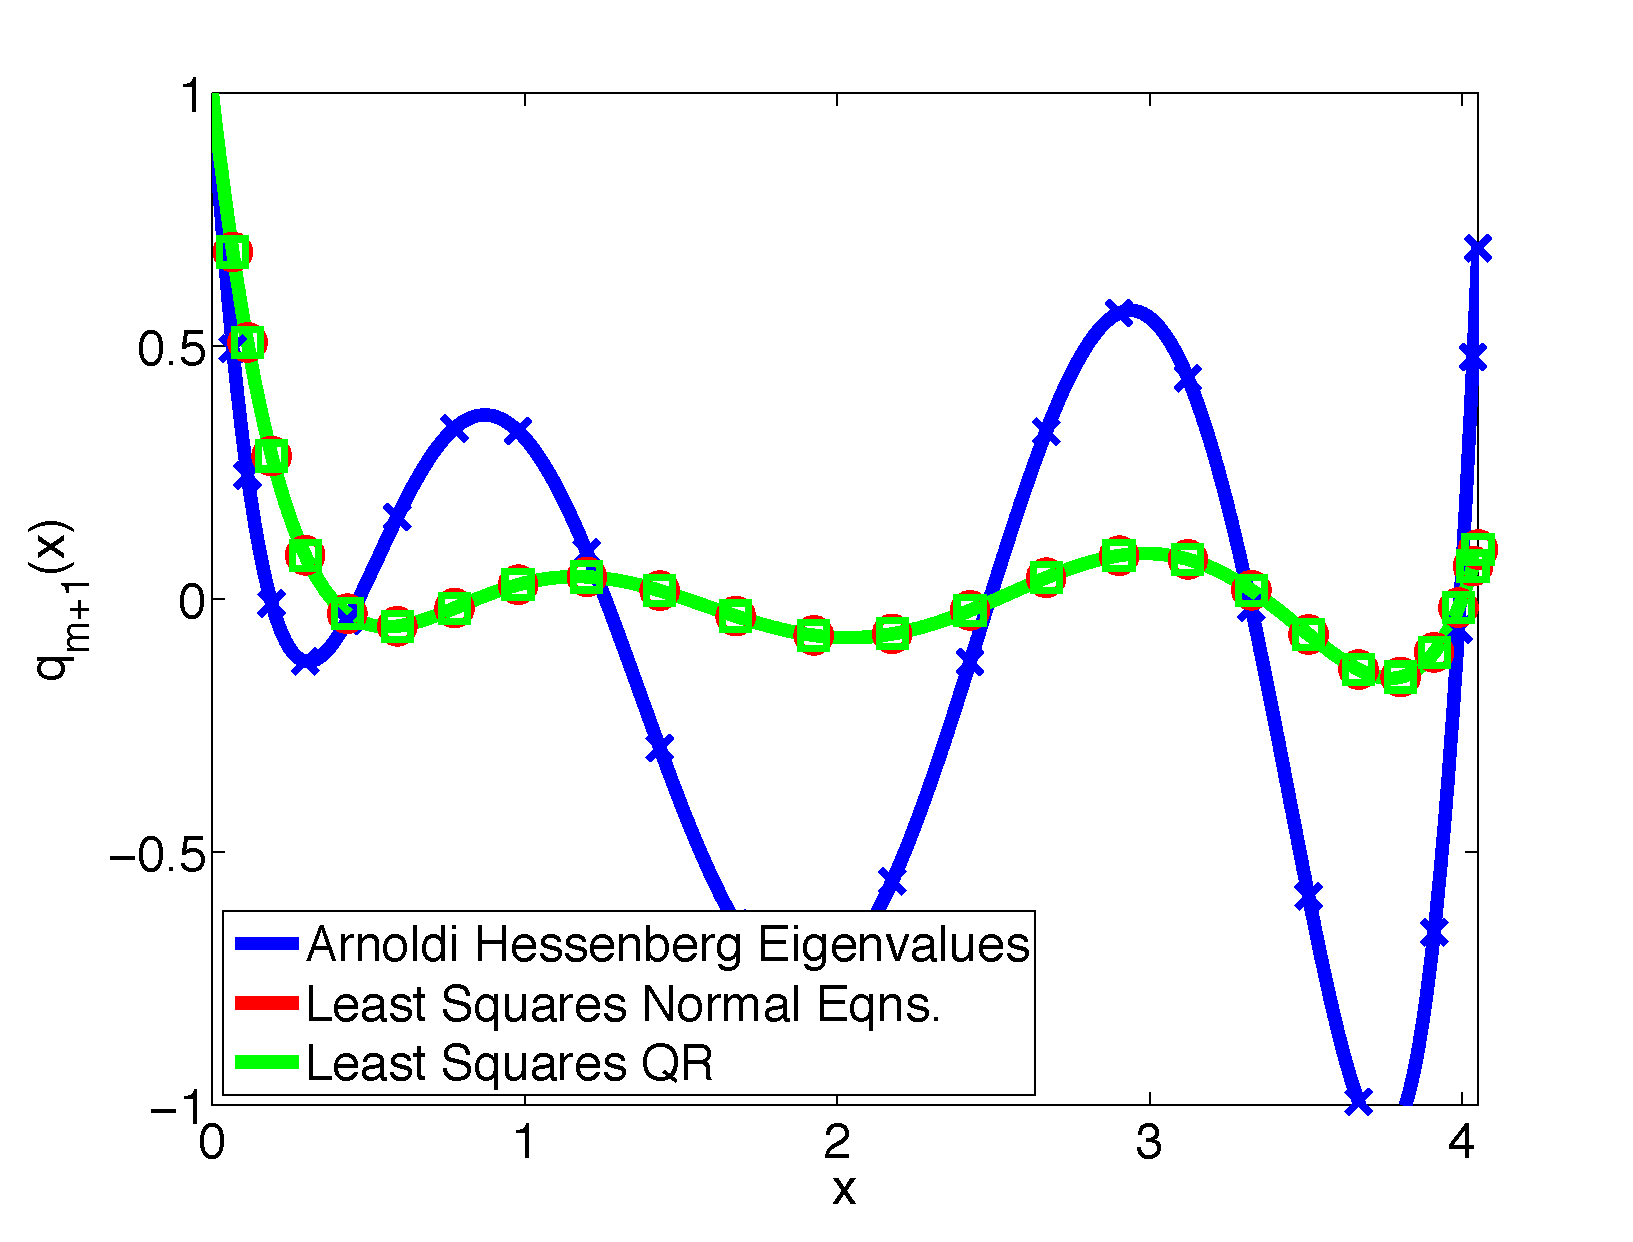
\includegraphics[width=\textwidth]{gmres_poly5}
\caption{$m = 5$}
\end{subfigure}
\begin{subfigure}[b]{0.49\linewidth}
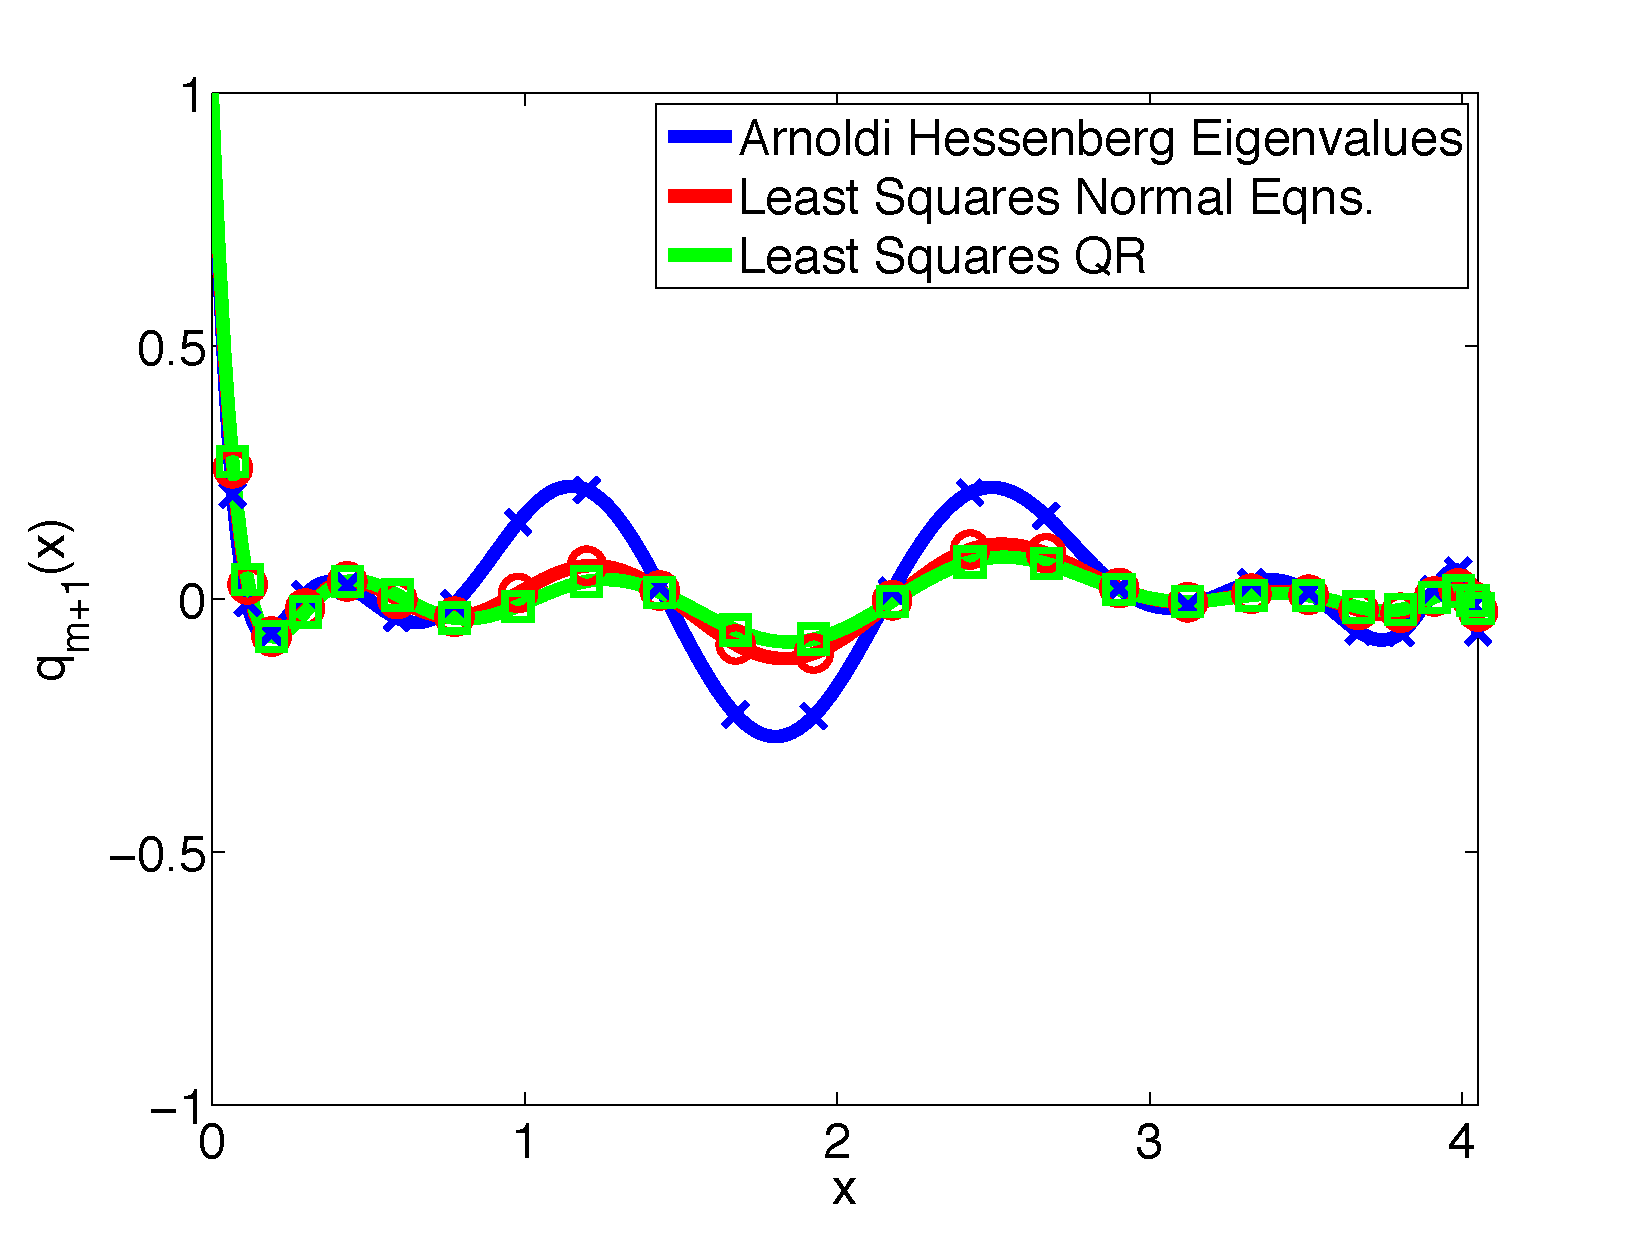
\includegraphics[width=\textwidth]{gmres_poly10}
\caption{$m = 10$}
\end{subfigure}
\begin{subfigure}[b]{0.49\linewidth}
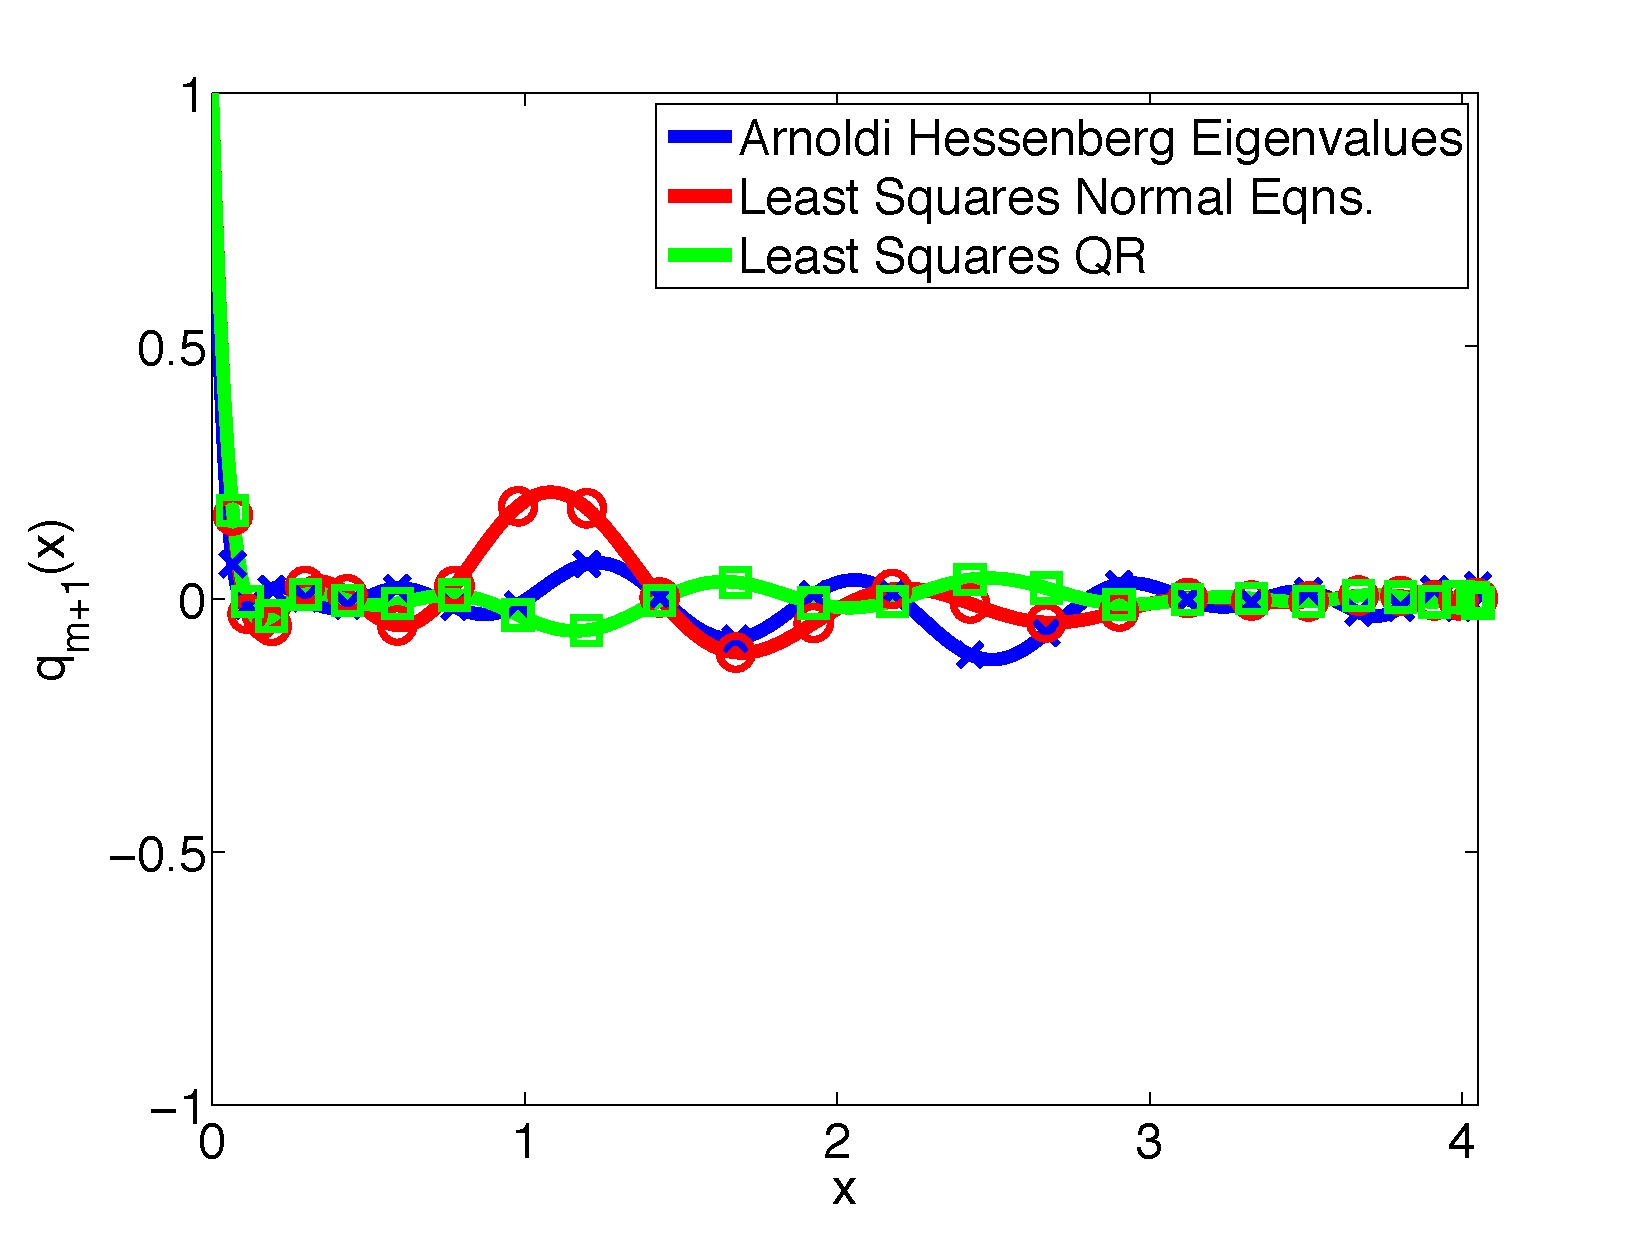
\includegraphics[width=\textwidth]{gmres_poly15}
\caption{$m = 15$}
\end{subfigure}
\begin{subfigure}[b]{0.49\linewidth}
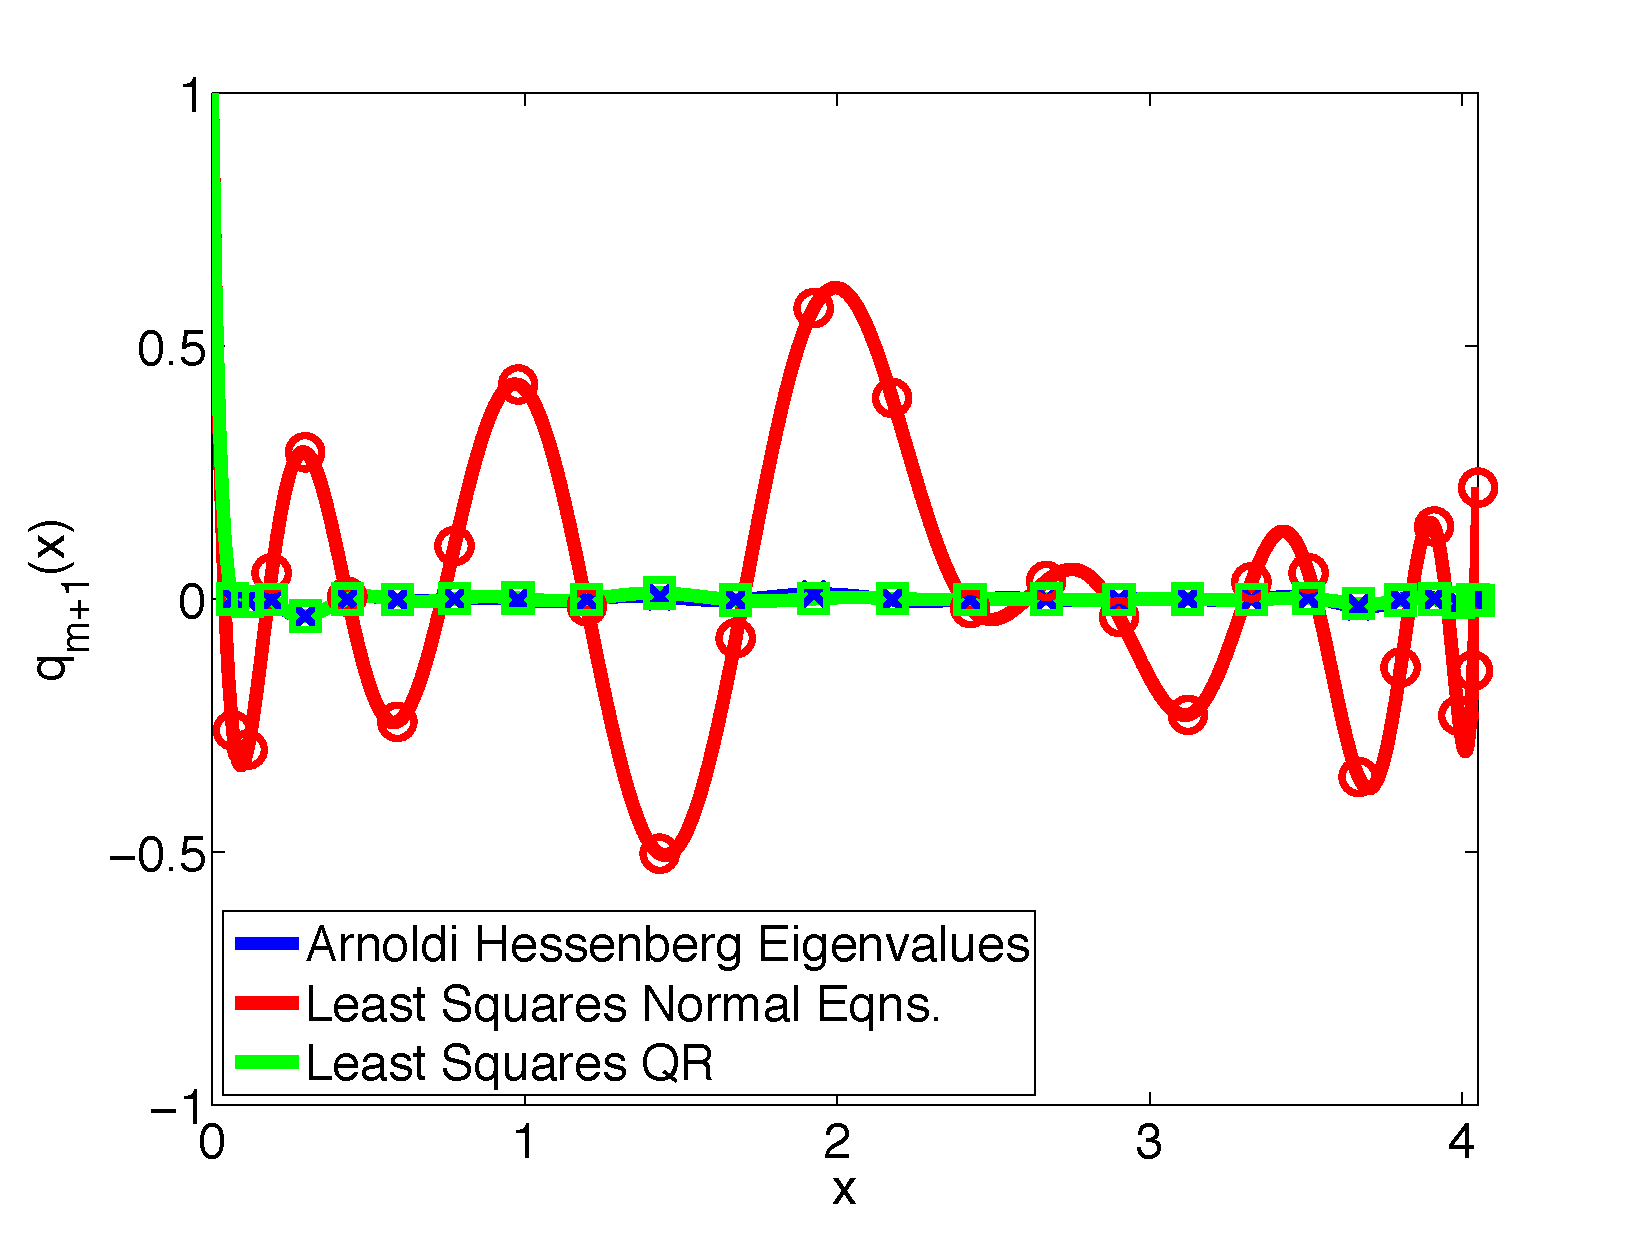
\includegraphics[width=\textwidth]{gmres_poly20}
\caption{$m = 20$}
\end{subfigure}
\caption{Plot of $q_{m+1}(x)=1-xp_{m}(x)$, where $p_m(x)$ is the GMRES
 polynomial with different methods for computing the coefficients.
 \bA\ is a shifted Laplacian with $N=25$.  Markers
 indicate the polynomials evaluated at the eigenvalues of \bA.}
\label{fig:gmres_poly}
\end{figure}

\begin{table}
\centering
\caption{Spectral Radius of $\left( \bI - p_m(\bA) \bA \right)$.}
\label{tab:gmres_poly}
\begin{tabular}{ccccc}
\toprule
& \multicolumn{4}{c}{Polynomial Order} \\
\cmidrule(r){2-5}
Method & 5 & 10 & 15 & 20 \\
\midrule
Hessenberg Eigenvalues     & 0.569 & 0.231 & 0.109 & 0.088 \\
Least Squares Normal Eqns. & 0.632 & 0.259 & 0.184 & 0.247 \\
Least Squares QR           & 0.632 & 0.273 & 0.176 & 0.586 \\
\bottomrule
\end{tabular}
\end{table}

\section{Results}
\label{sec:results}

As a simple test problem, we choose the ``JPWH 991'' matrix from
the Harwell-Boeing Collection, available from the Matrix Market.
The sparsity pattern of the JPWH matrix is given in Figure~\ref{fig:jpwh_sparsity}.
\begin{figure}
\centering
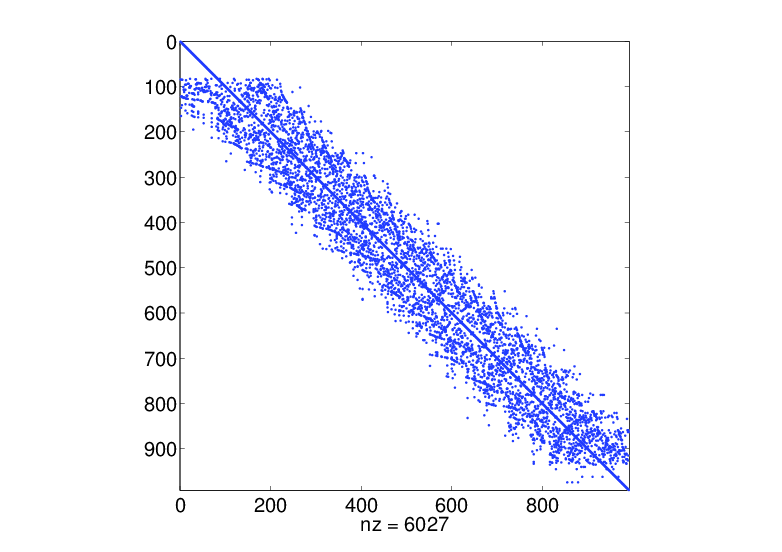
\includegraphics[width=4.5in]{jpwh_sparsity}
\caption{Sparsity pattern of JPWH matrix \label{fig:jpwh_sparsity}}
\end{figure}
The matrix is nonsymmetric, but its eigenvalues are all real and
contained in the interval $[-16.3,-0.12]$.  After a diagonal row
scaling, the eigenvalues are contained in the interval $[0.02,1.71]$.
All test cases use the diagonally scaled matrix and the right
hand side of the linear system is taken to be a vector of all ones.
The stopping criterion is a reduction in the L$_2$ norm of the residual
by six orders of magnitude.

Table~\ref{tab:jpwh_standard_neumann} shows the behavior of
the standard MCSA algorithm applied to the JPWH matrix for a range
of different polynomial orders and Monte Carlo histories per iteration.
As expected, increasing the polynomial order generally leads to a decrease
in the number of iterations required for convergence.
For a fixed number of histories, however, there is a threshold beyond
which an increase in the polynomial order actually leads to very slow
convergence or even divergence.  Conversely, for a fixed polynomial order
it is necessary to track ``enough'' histories to ensure stability, but
beyond that point there is little benefit to executing additional histories.
\begin{table}
\caption{Standard MCSA with Neumann Basis, JPWH Matrix.
\label{tab:jpwh_standard_neumann}}
\centering
\begin{tabular}{cccccccccc}
\toprule
Histories per & \multicolumn{9}{c}{Polynomial Order} \\
Iteration & 1 & 2 & 4 & 8 & 16 & 32 & 64 & 128 & 256 \\
\midrule
100 & 234 & 175 & 121 & 183 & - & - & - & - & - \\
200 & 230 & 173 & 118 & 74 & 164 & - & - & - & - \\
400 & 227 & 171 & 115 & 71 & 42 & 91 & - & - & - \\
800 & 227 & 170 & 114 & 70 & 39 & 31 & 47 & 67 & 78 \\
1600 & 226 & 170 & 113 & 69 & 39 & 22 & 22 & 27 & 27 \\
3200 & 225 & 169 & 113 & 68 & 38 & 21 & 15 & 17 & 17 \\
6400 & 225 & 169 & 113 & 68 & 38 & 21 & 12 & 12 & 13 \\
12800 & 225 & 169 & 113 & 68 & 38 & 21 & 11 & 10 & 10 \\
\bottomrule
\end{tabular}
\end{table}

Table~\ref{tab:jpwh_cheby_power} shows the same result,
but now instead of using $\bI - \bA$ as the basis for the
polynomial expansion, $\bA$ is used instead.
Thus, instead of Eq.~\eqref{eq:mc_decomp} defining the
matrices to be used in the Monte Carlo process, we instead
have
\begin{equation}
\bA^T = \bP \circ \bW \:.
\end{equation}
We see that
for this basis, the majority of cases result in divergence.
Interestingly, at low polynomial orders and large history
counts, the behavior is nearly identical to that with
$\bI - \bA$ as the basis.
\begin{table}
\caption{Standard MCSA with Monomial Basis, JPWH Matrix.
\label{tab:jpwh_standard_power}}
\centering
\begin{tabular}{cccccccccc}
\toprule
Histories per & \multicolumn{9}{c}{Polynomial Order} \\
Iteration & 1 & 2 & 4 & 8 & 16 & 32 & 64 & 128 & 256 \\
\midrule
    100 & -     & -     & - & - & - & - & - & - & - \\
    200 & 330 & -     & - & - & - & - & - & - & - \\
    400 & 240 & -     & - & - & - & - & - & - & - \\
    800 & 235 & 290 & - & - & - & - & - & - & - \\
  1600 & 230 & 182 & - & - & - & - & - & - & - \\
  3200 & 228 & 177 & - & - & - & - & - & - & - \\
  6400 & 227 & 174 & - & - & - & - & - & - & - \\
12800 & 226 & 172 & - & - & - & - & - & - & - \\
\bottomrule
\end{tabular}
\end{table}

Table~\ref{tab:jpwh_cheby_neumann} shows the performance
with Chebyshev polynomials rather than the Neumann
series.  Note that the polynomial order is increased
linearly in this case rather than exponentially with the
Neumann series.  In general, using Chebyshev polynomials
results in a significant reduction in iterations relative to
the equivalent order Neumann series polynomial.  The
downside is that significantly more histories must be
tracked to achieve stability for a given polynomial order.
\begin{table}
\caption{Chebyshev MCSA with Neumann Basis, JPWH Matrix.
\label{tab:jpwh_cheby_neumann}}
\centering
\begin{tabular}{cccccc}
 \toprule
 Histories per & \multicolumn{5}{c}{Polynomial Order} \\
 Iteration & 1 & 2 & 3 & 4 & 5 \\
 \midrule
 100 & - & - & - & - & - \\
 200 & 156 & - & - & - & - \\
 400 & 131 & - & - & - & - \\
 800 & 126 & 96 & - & - & - \\
 1600 & 125 & 67 & - & - & - \\
 3200 & 124 & 65 & 85 & - & - \\
 6400 & 123 & 64 & 42 & - & - \\
 12800 & 123 & 63 & 40 & 87 & - \\
 25600 & 123 & 63 & 40 & 33 & - \\
 51200 & 123 & 63 & 39 & 28 & 100 \\
 102400 & 122 & 63 & 39 & 28 & 33 \\
 204800 & 122 & 63 & 39 & 27 & 22 \\
\bottomrule
\end{tabular}
\end{table}

Table~\ref{tab:jpwh_cheby_power} shows the result of
again using Chebyshev polynomials, but now using
$\bA$ as the basis for the polynomial expansion.
As with the Neumann series polynomial, using
$\bA$ as a basis performs considerably worse than
using $\bI - \bA$ in that considerably more histories
are required to achieve stability for a given polynomial
order.
\begin{table}
\caption{Chebyshev MCSA with Monomial Basis, JPWH Matrix.
\label{tab:jpwh_cheby_power}}
\centering
\begin{tabular}{cccccc}
 \toprule
 Histories per & \multicolumn{5}{c}{Polynomial Order} \\
 Iteration & 1 & 2 & 3 & 4 & 5 \\
 \midrule
 100 & - & - & - & - & - \\
 200 & - & - & - & - & - \\
 400 & - & - & - & - & - \\
 800 & - & - & - & - & - \\
 1600 & 178 & - & - & - & - \\
 3200 & 130 & - & - & - & - \\
 6400 & 127 & - & - & - & - \\
 12800 & 125 & - & - & - & - \\
 25600 & 124 & 80 & - & - & - \\
 51200 & 123 & 67 & - & - & - \\
 102400 & 123 & 65 & - & - & - \\
 204800 & 123 & 64 & - & - & - \\
\bottomrule
\end{tabular}
\end{table}

\bibliographystyle{plain}
\bibliography{references}

\end{document}
